\section{Параллельные и расходящиеся прямые}

\subsection{Параллельные прямые в модели}

Прямые будем считать направленными: направление задаётся упорядоченной парой точек, $a=A_1A_2$.

\begin{definition}[\!\!{[1,~2]}]
Направленная прямая $b=B_1B_2$ называется \emph{параллельной} прямой $a$, если $a$ и $b$ не пересекаются и для любых точек $A\in a$, $B\in b$ любой внутренний луч угла $ABB_2$ пересекает $a$.
\end{definition}

В абсолютной геометрии доказывается~[1], что условие достаточно проверить для одной пары точек $A$, $B$, что через каждую точку вне прямой проходит ровно одна прямая, параллельная ей в данном направлении, и что параллельность симметрична и транзитивна. Модель делает эти утверждения наглядными.

\begin{theorem}\label{thm:parallel-model}
Направленная π-прямая $b=B_1B_2$ параллельна π-прямой $a$ тогда и только тогда, когда конец хорды $b$ в направлении $B_2$ является одним из концов хорды $a$.
\end{theorem}
\begin{proof}
Пусть конец $\Omega$ хорды $b$ в направлении $B_2$ лежит на $a$. Хорды $a$ и $b$ имеют одну общую точку $\Omega$, и она не является π-точкой, поэтому π-прямые не пересекаются. Пусть $A\in a$, $B\in b$ и $h$~--- внутренний луч угла $AB\Omega$. Концы евклидова отрезка $A\Omega$ лежат на сторонах этого угла, поэтому $h$ пересекает отрезок $A\Omega$ во внутренней точке. Эта точка лежит внутри круга и принадлежит $a$.

Обратно, пусть $b$ параллельна $a$, а конец $V$ хорды $b$ в направлении $B_2$ не является концом $a$. Возьмём $A\in a$, $B\in b$. Прямая $AB$ пересекает хорду $a$ в точке $A$, поэтому концы хорды $a$ лежат по разные стороны от прямой $AB$; обозначим через $U$ тот из них, который лежит по одну сторону с $V$. Лучи $BU$ и $BV$ различны. Если луч $BU$ внутренний для угла $ABV$, то он не пересекает $a$ (прямая, содержащая хорду $a$, встречает его только в точке $U$ абсолюта), что противоречит определению. Если же луч $BV$ внутренний для угла $ABU$, то он пересекает отрезок $AU$ во внутренней точке, и прямые $a$ и $b$ пересекаются. Оба случая невозможны.
\end{proof}

Из теоремы~\ref{thm:parallel-model} сразу следуют свойства параллельных, которые в абсолютной геометрии требуют отдельных доказательств~[1]. Через π-точку $B$ вне прямой $a$ проходят ровно две прямые, параллельные $a$: хорды, соединяющие $B$ с концами хорды $a$. Параллельность в фиксированном направлении означает, что хорды имеют один и тот же конец в этом направлении, поэтому она симметрична и транзитивна: если $a$ и $b$ идут в точку $\Omega$ абсолюта, а $b$ и $c$ идут в ту же точку $\Omega$, то и $a$ с $c$ идут в $\Omega$. Для отношения «иметь какой-нибудь общий конец» транзитивность неверна: хорды $\Omega_1\Omega_2$ и $\Omega_1\Omega_3$ имеют общий конец, хорды $\Omega_1\Omega_3$ и $\Omega_3\Omega_4$ тоже, а хорды $\Omega_1\Omega_2$ и $\Omega_3\Omega_4$ его не имеют. Поэтому параллельность всегда рассматривают в определённом направлении. Две различные хорды имеют не больше одного общего конца, поэтому если $A_1A_2\parallel B_1B_2$, то $B_2B_1$ не параллельна $A_2A_1$. Аксиома Лобачевского в модели выполняется: через $B$ проходят по крайней мере две прямые, не пересекающие $a$, и все хорды, лежащие в вертикальных углах между двумя параллельными и не содержащие $a$, тоже её не пересекают.

\subsection{Угол параллельности и формула Лобачевского}

\begin{definition}[\!\!{[1]}]
Пусть $BH$~--- перпендикуляр к прямой $a$, а прямая $b$ проходит через $B$ и параллельна $a$. Угол между лучом $BH$ и прямой $b$ (в направлении параллельности) называется \emph{углом параллельности} отрезка $BH$.
\end{definition}

Равным отрезкам соответствуют равные углы параллельности, поэтому угол параллельности зависит только от длины $x=BH$. Эта зависимость $\Pi(x)$ называется \emph{функцией Лобачевского}. В модели её можно вычислить, если поместить вершину угла в центр круга.

\begin{theorem}\label{thm:lobachevsky}
Для любого $x>0$
\begin{equation}\label{eq:lobachevsky}
\cos\Pi(x)=\thh x,\qquad\text{или, что равносильно,}\qquad \operatorname{tg}\frac{\Pi(x)}{2}=e^{-x}.
\end{equation}
\end{theorem}
\begin{proof}
Переведём π-движением точку $B$ в центр $O$, а точку $H$~--- в точку $(0,-\eta)$ отрицательной полуоси ординат. По следствию~\ref{cor:ot-centra} $\eta=\thh x$. Прямая $a$ перпендикулярна диаметру $BH$ в точке $H$, поэтому по лемме~\ref{lem:polyus} она изображается евклидово перпендикулярной хордой $k_2=-\eta$ с концами $\bigl(\pm\sqrt{1-\eta^2},\,-\eta\bigr)$. Прямые, проходящие через $O$ и параллельные $a$, по теореме~\ref{thm:parallel-model} соединяют $O$ с этими концами. Угол между ними и лучом $OH$ имеет вершину в центре и изображается без искажения (предложение~\ref{prop:ugol}), а его косинус равен
\[
\cos\Pi(x)=\frac{(0,-1)\cdot(\sqrt{1-\eta^2},\,-\eta)}{1}=\eta=\thh x.
\]
Наконец, $\operatorname{tg}^2\frac{\Pi}{2}=\frac{1-\cos\Pi}{1+\cos\Pi}=\frac{1-\thh x}{1+\thh x}=e^{-2x}$.
\end{proof}

\begin{figure}[H]
\centering
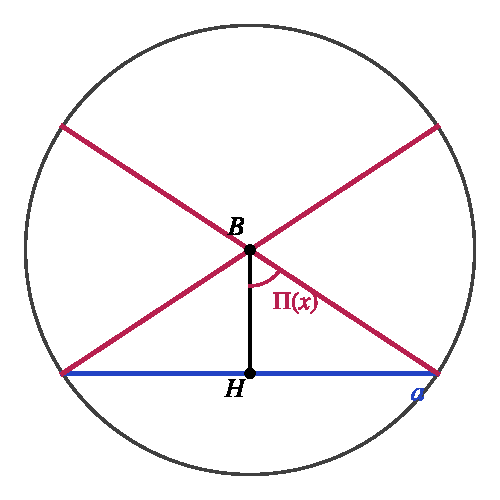
\includegraphics[width=0.46\textwidth]{fig/pi.pdf}
\caption{Угол параллельности отрезка $BH$ при вершине $B$ в центре круга: прямые через $B$, параллельные $a$, идут в концы хорды $a$}
\label{fig:pi}
\end{figure}

Из формулы~\eqref{eq:lobachevsky} видны свойства функции Лобачевского, которые в курсе доказываются с помощью аксиомы Дедекинда. Функция $\Pi(x)$ непрерывна и строго убывает; при $x\to0$ угол стремится к прямому, при $x\to\infty$~--- к нулю. Каждый острый угол $\varphi$ является углом параллельности отрезка длины $x=\operatorname{arth}(\cos\varphi)$. Несколько значений приведены в таблице~\ref{tab:pi}.

\begin{table}[H]
\caption{Значения функции Лобачевского}
\label{tab:pi}
\centering
\begin{tabular}{|c|c|c|c|c|c|}
\hline
$x$ & $0{,}1$ & $0{,}5$ & $1$ & $2$ & $3$ \\ \hline
$\Pi(x)$ & $84{,}28^\circ$ & $62{,}48^\circ$ & $40{,}40^\circ$ & $15{,}41^\circ$ & $5{,}70^\circ$ \\ \hline
\end{tabular}
\end{table}

\subsection{Взаимное расположение двух прямых и общий перпендикуляр}

\begin{definition}[\!\!{[1]}]
Две прямые плоскости Лобачевского называются \emph{расходящимися}, если они не пересекаются и не параллельны.
\end{definition}

Пусть $a$ и $b$~--- различные π-прямые, $X$~--- точка пересечения содержащих их евклидовых прямых (если эти прямые параллельны, $X$~--- бесконечно удалённая точка). По теореме~\ref{thm:parallel-model} прямые $a$ и $b$ пересекаются, если $X$ лежит внутри круга, параллельны, если $X$ лежит на абсолюте, и расходятся, если $X$ лежит вне круга (рисунок~\ref{fig:klassifikaciya}).

\begin{figure}[H]
\centering
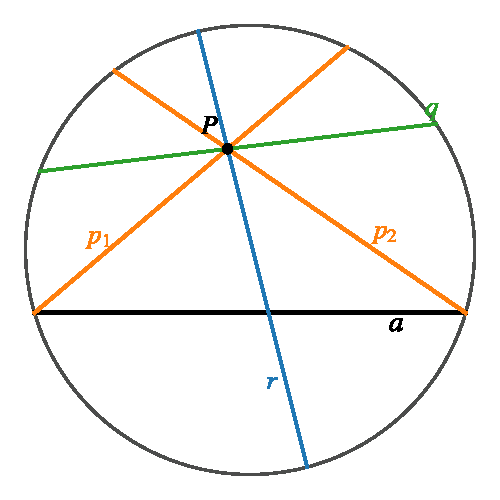
\includegraphics[width=0.48\textwidth]{fig/klassifikaciya.pdf}
\caption{Прямые, проходящие через точку $P$: $r$ пересекает прямую $a$, $p_1$ и $p_2$ ей параллельны, $q$ с ней расходится}
\label{fig:klassifikaciya}
\end{figure}

\begin{theorem}[признак расходящихся прямых]\label{thm:perpendikulyar}
Две непересекающиеся прямые расходятся тогда и только тогда, когда у них есть общий перпендикуляр. Общий перпендикуляр расходящихся прямых единствен; в модели это хорда, проходящая через полюсы обеих прямых.
\end{theorem}
\begin{proof}
Пусть $P_a$ и $P_b$~--- полюсы прямых $a$ и $b$. По лемме~\ref{lem:polyus} прямая перпендикулярна и $a$, и $b$ тогда и только тогда, когда она проходит через $P_a$ и $P_b$, то есть совпадает с евклидовой прямой $P_aP_b$. Точка $X$ лежит на поляре точки $P_a$ (это прямая $a$) и на поляре $P_b$, поэтому по взаимности полюса и поляры прямая $P_aP_b$ есть поляра точки $X$. Если $X$ вне круга, её поляра пересекает круг и даёт единственный общий перпендикуляр. Если $X$ на абсолюте, её поляра~--- касательная, и общего перпендикуляра нет. Если $X$ внутри круга, поляра не пересекает круг; этот случай пересекающихся прямых условием исключён.
\end{proof}

Так в модели выглядит построение общего перпендикуляра: провести касательные к абсолюту в концах обеих хорд, найти два полюса и соединить их. Длину общего перпендикуляра тоже можно найти по полюсам.

\begin{proposition}\label{prop:ch-rasstoyaniya}
Если $a$ и $b$ расходятся, а $\delta$~--- длина их общего перпендикуляра, то
\[
\frac{|\sk{P_a}{P_b}|}{\sqrt{\sk{P_a}{P_a}\sk{P_b}{P_b}}}=\ch\delta.
\]
Для пересекающихся прямых та же величина равна $|\cos\varphi|$ (предложение~\ref{prop:ugol}), для параллельных она равна $1$.
\end{proposition}
\begin{proof}
Величина не меняется при π-движениях. Переведём основание общего перпендикуляра на $a$ в центр, а сам перпендикуляр~--- на ось ординат. Тогда $a$~--- диаметр $k_2=0$ с полюсом $(0:0:1)$, а $b$ перпендикулярна оси ординат и изображается хордой $k_2=c$ с полюсом $(c:0:1)$, где $\delta=\operatorname{arth}|c|$ по следствию~\ref{cor:ot-centra}. Подстановка в~\eqref{eq:forma} даёт $1/\sqrt{1-c^2}=\ch\delta$. Для параллельных прямых поместим общий конец в точку $(1,0)$, а прямую $a$ на диаметр $k_2=0$. Тогда $b$ изображается хордой $\kappa-\kappa k_1-k_2=0$ с полюсом $(\kappa:\kappa:1)$, и $\sk{P_a}{P_b}=1$, $\sk{P_a}{P_a}=1$, $\sk{P_b}{P_b}=-\kappa^2+\kappa^2+1=1$.
\end{proof}

\subsection{Расстояние от точек прямой до другой прямой}

\begin{proposition}\label{prop:do-diametra}
Расстояние $d$ от π-точки $(x,y)$ до диаметра $k_2=0$ определяется равенством
\begin{equation}\label{eq:do-diametra}
\thh d=\frac{|y|}{\sqrt{1-x^2}}.
\end{equation}
\end{proposition}
\begin{proof}
По лемме~\ref{lem:polyus} перпендикуляр из точки $M=(x,y)$ к диаметру изображается вертикальной хордой, его основание $F=(x,0)$. По предложению~\ref{prop:ch}
\[
\ch d(M,F)=\frac{1-x^2}{\sqrt{(1-x^2)(1-x^2-y^2)}}=\sqrt{\frac{1-x^2}{1-x^2-y^2}},
\]
откуда $\thh^2d=1-\dfrac{1}{\ch^2d}=\dfrac{y^2}{1-x^2}$.
\end{proof}

С помощью этой формулы теоремы о расстоянии между точками двух прямых~[1] получают явный вид. Будем двигать точку $M$ по прямой $b$ и следить за её расстоянием до прямой $a$, которую π-движением поместим на диаметр $k_2=0$.

\emph{Параллельные прямые.} Пусть $b$ параллельна $a$ в направлении конца $(1,0)$. Тогда $b$ изображается хордой $y=\kappa(1-x)$, $\kappa\ne0$, и по~\eqref{eq:do-diametra}
\[
\thh d=|\kappa|\,\frac{1-x}{\sqrt{1-x^2}}=|\kappa|\sqrt{\frac{1-x}{1+x}}.
\]
Эта величина строго убывает с ростом $x$, стремится к нулю при $x\to1$ и стремится к единице, то есть $d\to\infty$, когда $M$ уходит к другому концу хорды $b$. Значит, расстояние от точки одной из параллельных прямых до другой неограниченно убывает в направлении параллельности, неограниченно возрастает в противоположном направлении и принимает любое положительное значение ровно один раз.

\emph{Расходящиеся прямые.} Поместим общий перпендикуляр на ось ординат. Прямая $b$ перпендикулярна этой оси и изображается хордой $y=c$, $0<|c|<1$:
\[
\thh d=\frac{|c|}{\sqrt{1-x^2}},\qquad |x|<\sqrt{1-c^2}.
\]
Наименьшее значение $|c|$ достигается при $x=0$, то есть в основании общего перпендикуляра, и равно $\thh\delta$. При удалении $M$ от общего перпендикуляра в любую сторону расстояние неограниченно возрастает (рисунок~\ref{fig:rasstoyanie}).

\begin{figure}[H]
\centering
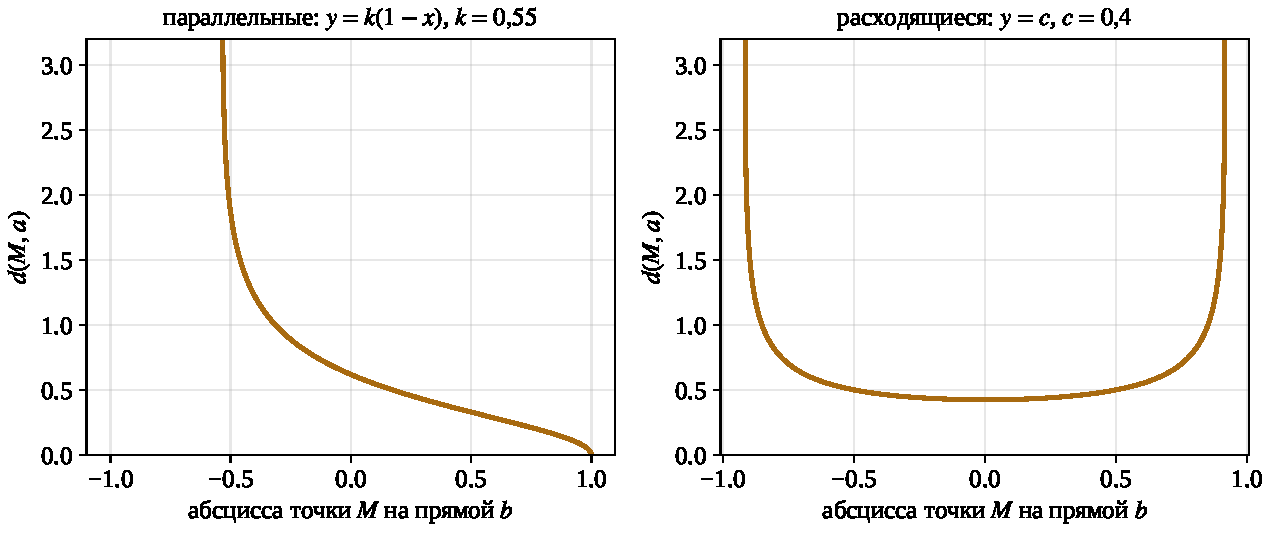
\includegraphics[width=\textwidth]{fig/rasstoyanie.pdf}
\caption{Расстояние от точки $M$ прямой $b$ до прямой $a$ (диаметра $k_2=0$): слева $b$ параллельна $a$, справа расходится с ней}
\label{fig:rasstoyanie}
\end{figure}

В евклидовой геометрии ни того, ни другого поведения нет: точка прямой, параллельной данной, остаётся на одном расстоянии от неё. В интерактивной модели этому посвящена сцена «Общий перпендикуляр и расстояние»: при перетаскивании концов хорды $b$ график расстояния переходит от U-образной кривой к монотонной в тот момент, когда концы хорд совпадают.
